\chapter{HASIL DAN PEMBAHASAN} \label{cha:4-HasilDanPembahasan}

\section{Hasil Pemelajaran Model} \label{sec:4-PersiapanPengujian}

Pemelajaran model yang dilakukan selama sepuluh \textit{epochs} menunjukkan bahwa kesalahan model
dalam mengestimasi pose tiga dimensi berkurang dalam setiap \textit{epoch}. \text{Learning rate}
yang dibagi dua dalam setiap \textit{epoch} mempengaruhi pemelajaran model dimana penyesuaian model
semakin teliti. Adaptasi bobot model terjadi secara drastis pada \textit{epoch} 0 sampai dengan
\textit{epoch} 3. \textit{Epoch} 4 dan seterusnya menggunakan \textit{learning rate} yang semakin
kecil sehingga model semakin teliti dalam melakukan adaptasi. Grafik pemelajaran model dapat dilihat
pada gambar~\ref{fig:pelatihan}.

\begin{figure}[htbp]
    \begin{center}
        \fbox{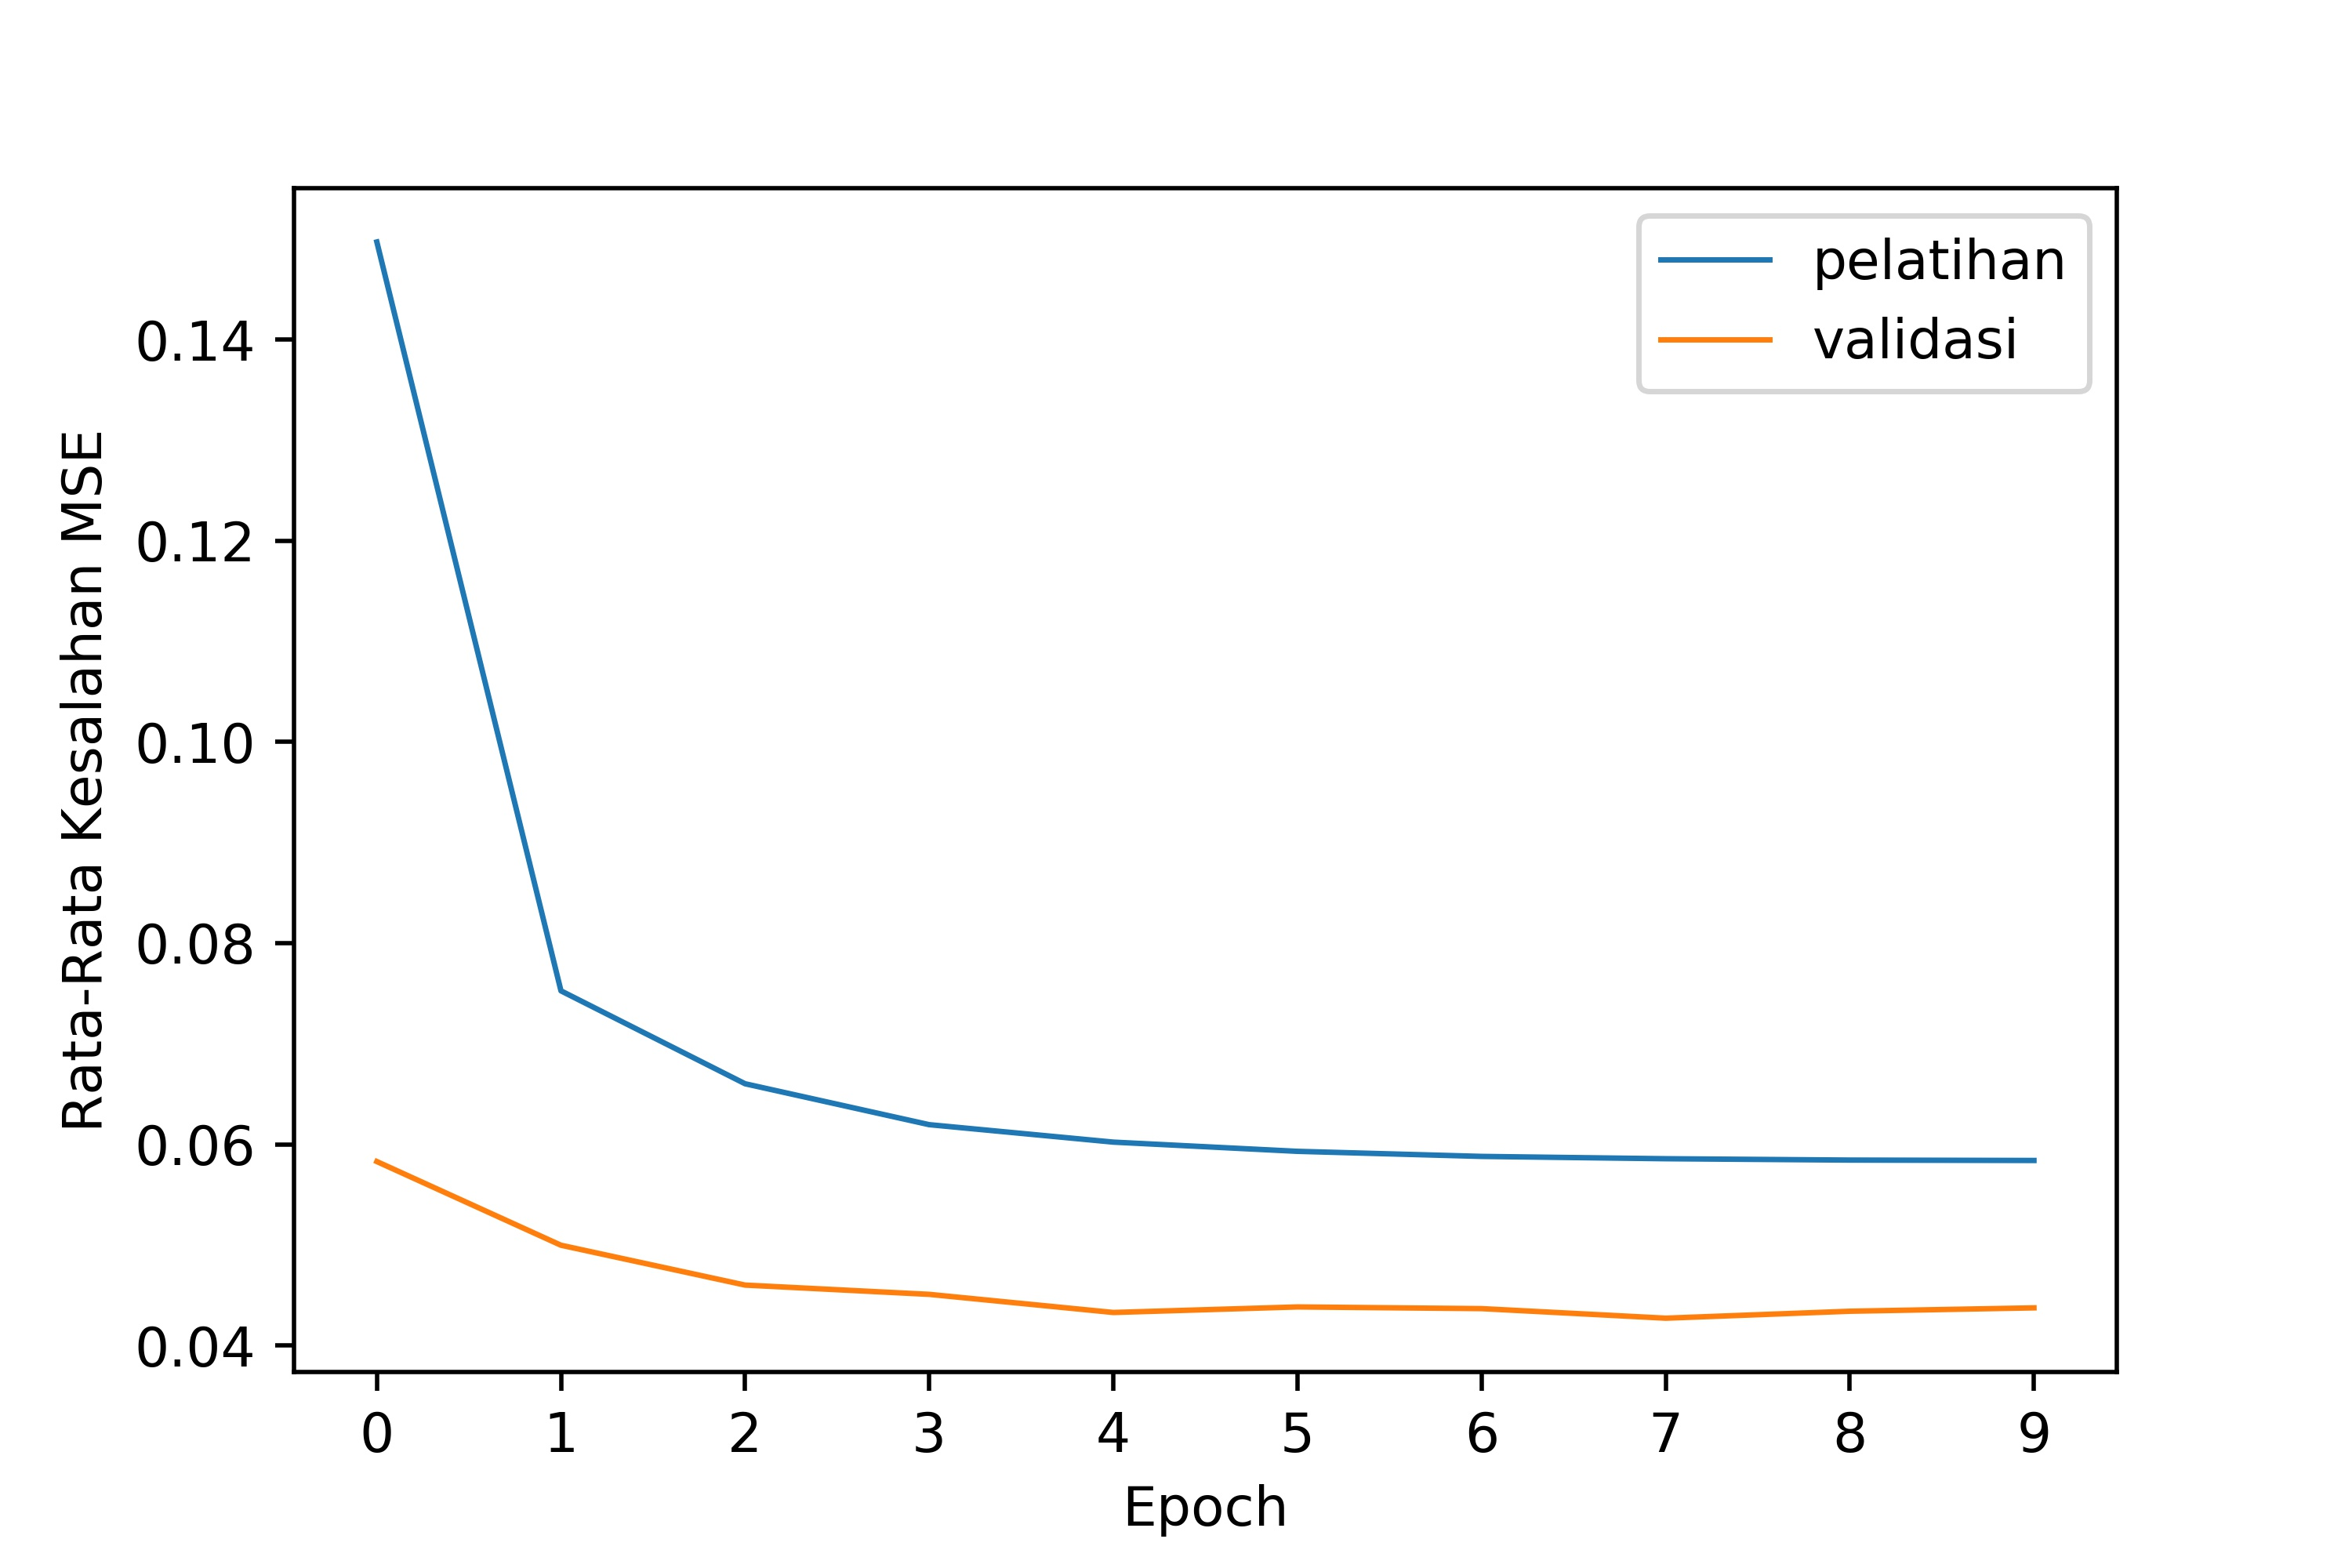
\includegraphics[width=11.9cm]{bab4/gambar/pelatihan.jpg}}
    \end{center}
    \vspace{-20pt}
    \captionsetup{labelfont=bf, textfont=bf}
    \caption{Grafik Pemelajaran Model}
    \vspace{-10pt}
    \captionsetup{labelfont=md, textfont=md}
    % \caption*{Sumber: sumber}
    % \caption*{Sumber: nama(2019)}
    \label{fig:pelatihan}
\end{figure}

\section{Analisis Uji Coba Aplikasi} \label{sec:4-PersiapanPengujian}

Inferensi yang bagus akan terjadi apabila langkah-langkah pada tahapan uji coba tidak mengalami
kesalahan. Kualitas gambar dan pose yang tidak cacat juga mempengaruhi proses dari awal hingga akhir.
Prapemrosesan gambar pada data inferensi yang tepat memudahkan OpenPose dalam mencari titik kunci
pose dua dimensi secara lengkap. Titik kunci OpenPose yang lengkap kemudian memenuhi syarat untuk
dikonversi menjadi spesifikasi yang diinginkan. Informasi tersebut kemudian diteruskan ke model
untuk mendapatkan titik kunci pose tiga dimensi.
% Rangkaian langkah-langkah yang baik menghasilkan
% pose tiga dimensi yang realistis seperti pada gambar~\ref{fig:bro75}.

% \begin{figure}[htbp]
%     \begin{center}
%         \fbox{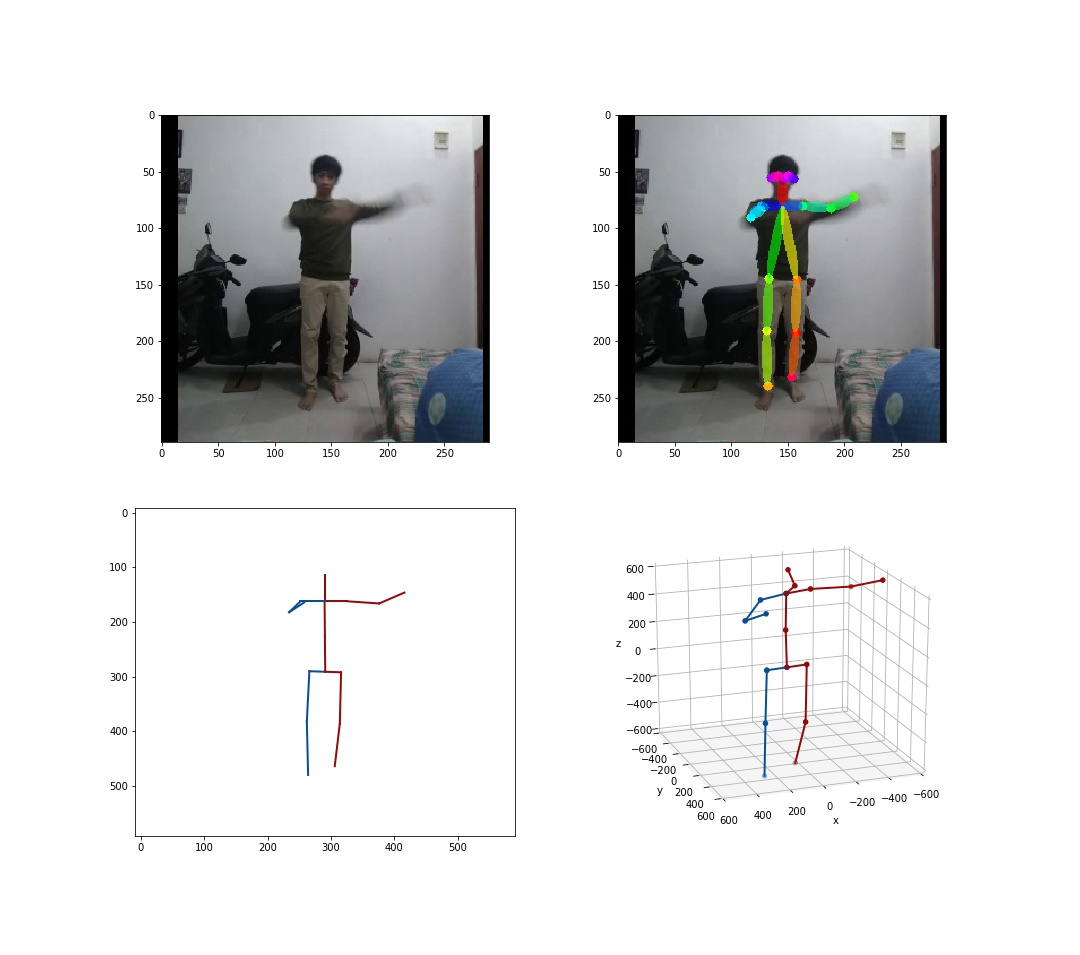
\includegraphics[width=11.9cm]{bab4/gambar/bro75.jpg}}
%     \end{center}
%     \vspace{-20pt}
%     \captionsetup{labelfont=bf, textfont=bf}
%     \caption{Inferensi Tepat}
%     \vspace{-10pt}
%     \captionsetup{labelfont=md, textfont=md}
%     % \caption*{Sumber: sumber}
%     % \caption*{Sumber: nama(2019)}
%     \label{fig:bro75}
% \end{figure}

Kualitas pose yang cacat menghasilkan estimasi pose tiga dimensi yang cacat. Oklusi pose pada gambar
dua dimensi dapat menghilangkan suatu bagian tubuh. Hilangnya bagian ini dari gambar menyebabkan
kesalahan pada langkah-langkah selanjutnya. Titik kunci lengan kanan hilang ketika pose lengan
mengarah lurus ke lensa kamera sehingga terjadi oklusi. Hal ini menyebabkan OpenPose tidak dapat
menemukan titik kunci lengan kanan dan memberi nilai nol pada titik kunci tersebut. Proses konversi
dan inferensi titik kunci tiga dimensi juga menghasilkan pose yang tidak realistis. Inferensi pose
hilang yang diakibatkan oklusi dapat dilihat pada gambar~\ref{fig:bro76}.

\begin{figure}[htbp]
    \begin{center}
        \fbox{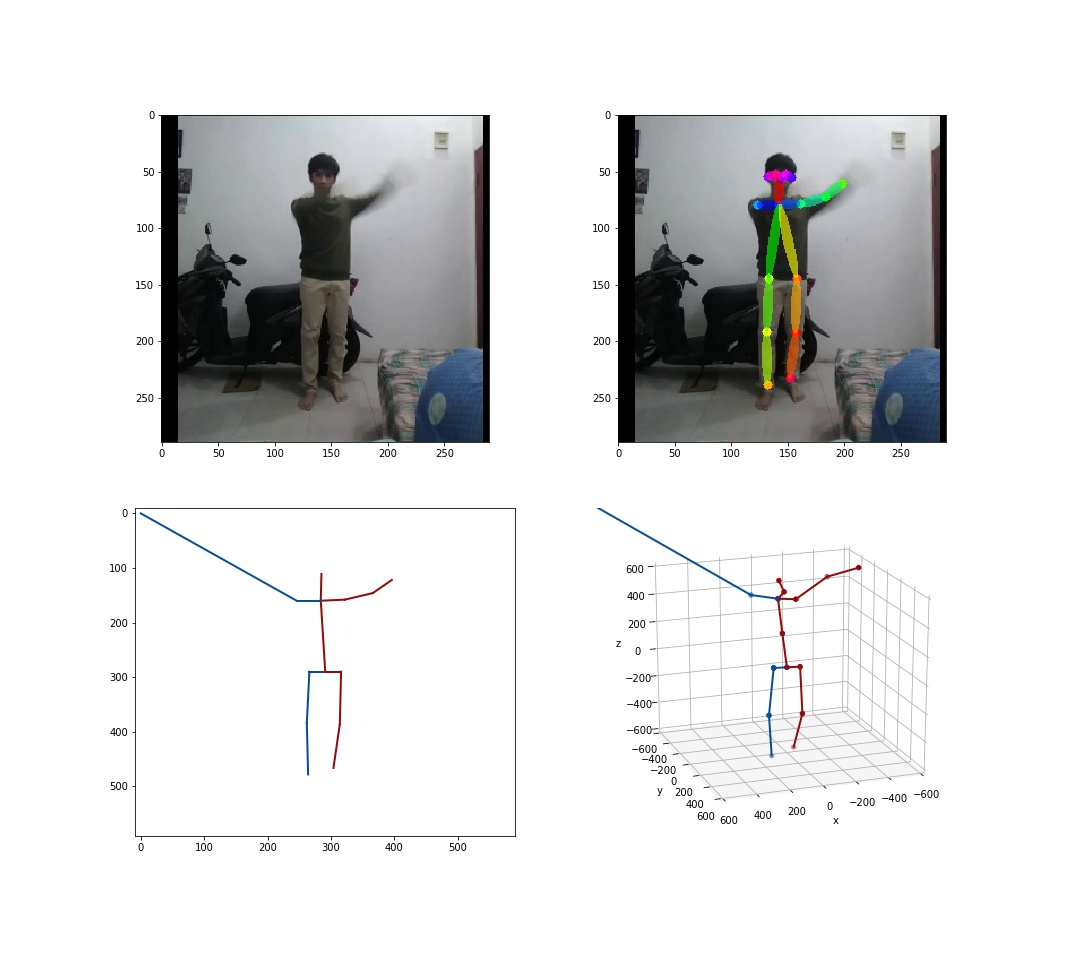
\includegraphics[width=11.9cm]{bab4/gambar/bro76.jpg}}
    \end{center}
    \vspace{-20pt}
    \captionsetup{labelfont=bf, textfont=bf}
    \caption{Inferensi Pose Hilang}
    \vspace{-10pt}
    \captionsetup{labelfont=md, textfont=md}
    % \caption*{Sumber: sumber}
    % \caption*{Sumber: nama(2019)}
    \label{fig:bro76}
\end{figure}

\pagebreak

Kesalahan juga dapat terjadi pada proses inferensi titik kunci. Apabila OpenPose mengeluarkan
\textit{output} yang ambigu dimana terdapat titik kunci yang dianggap sebagai bagian dari tubuh manusia.
OpenPose menghasilkan titik kunci ganda yang tidak sesuai dengan spesifikasi yang diperlukan meskipun
berhasil mendeteksi pose secara lengkap.
Hasil keluaran yang tidak sesuai dengan spesifikasi model mengakibatkan estimasi pose tiga dimensi yang rusak.
Inferensi pose yang mengalami kesalahan deteksi dapat dilihat pada gambar~\ref{fig:bro131}.

\begin{figure}[htbp]
    \begin{center}
        \fbox{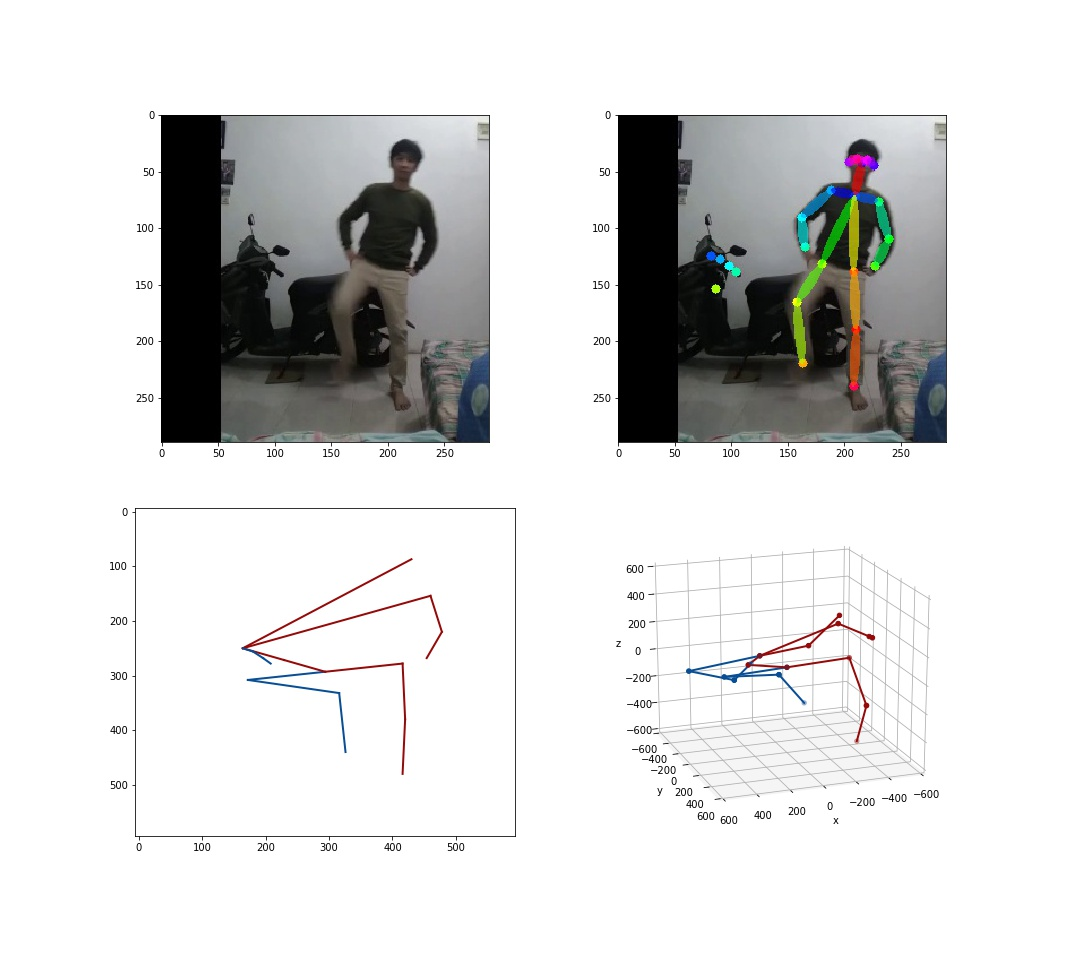
\includegraphics[width=11.9cm]{bab4/gambar/bro131.jpg}}
    \end{center}
    \vspace{-20pt}
    \captionsetup{labelfont=bf, textfont=bf}
    \caption{Kesalahan Deteksi}
    \vspace{-10pt}
    \captionsetup{labelfont=md, textfont=md}
    % \caption*{Sumber: sumber}
    % \caption*{Sumber: nama(2019)}
    \label{fig:bro131}
\end{figure}

\pagebreak

Akurasi estimasi pose tiga dimensi yang terjadi pada masukkan video uji coba dapat dianalisis
lebih mendalam.
Setiap titik kunci memiliki peran kontribusi terhadap estimasi pose secara keseluruhan. Analisis
setiap titik kunci secara tersendiri dilakukan dengan
pemberian nama kode.
Kode-kode terdiri dari lima belas titik kunci yang diwakilkan dengan kode huruf kapital terurut seperti pada
tabel \ref{tab:definisititikkunci} untuk mempermudah analisis.

\begin{table}[htbp]
    \captionsetup{labelfont=bf, textfont=bf}
    \caption{Definisi Titik Kunci}
    \label{tab:definisititikkunci}
    \vspace{-20pt}
    \begin{center}
        \begin{tabular}{|c|c|l|}
            \hline
            \textbf{No.} & \textbf{Kode} & \hspace{2cm}\textbf{Titik Kunci} \\ \hline
            1            & A             & Pinggang                         \\ \hline
            2            & B             & Paha Kanan                       \\ \hline
            3            & C             & Lutut Kanan                      \\ \hline
            4            & D             & Pergelangan Kaki Kanan           \\ \hline
            5            & E             & Paha Kiri                        \\ \hline
            6            & F             & Lutut Kiri                       \\ \hline
            7            & G             & Pergelangan Kaki Kiri            \\ \hline
            8            & H             & Leher                            \\ \hline
            9            & I             & Bahu Kanan                       \\ \hline
            10           & J             & Siku Kanan                       \\ \hline
            11           & K             & Pergelangan Tangan Kanan         \\ \hline
            12           & L             & Bahu Kiri                        \\ \hline
            13           & M             & Siku Kiri                        \\ \hline
            14           & N             & Pergelangan Tangan Kiri          \\ \hline
            15           & O             & Kepala                           \\ \hline
        \end{tabular}
    \end{center}
    \vspace{-10pt}
\end{table}

Hasil uji akurasi estimasi pose untuk setiap pose ditampilkan pada tabel \ref{tab:hasilujiakurasiestimasipose}.
Setiap kode titik kunci yang diisi dengan angka "1" mewakili akurasi estimasi yang benar
sedangkan angka "0" mewakili kesalahan estimasi pada titik kunci tersebut.
Keberadaan kuantitas estimasi yang benar dikalikan dengan banyaknya jumlah frame untuk mendapatkan
total estimasi. Kuantitas benarnya setiap titik kunci juga dijumlahkan sehingga pada akhirnya
didapatkan persentase estimasi setiap titik kunci terhadap estimasi secara keseluruhan.

\pagebreak

\begin{table}[htbp]
    \captionsetup{labelfont=bf, textfont=bf}
    \caption{Hasil Uji Akurasi Estimasi Pose}
    \label{tab:hasilujiakurasiestimasipose}
    \vspace{-20pt}
    \begin{center}
        \resizebox{\textwidth}{!}{\begin{tabular}{|l|l|c|c|c|c|c|c|c|c|c|c|c|c|c|c|c|c|}
                \hline
                \textbf{No.}                              & \multicolumn{17}{c|}{\textbf{Kode Titik Kunci}}                                                                                                                                                                                                                   \\
                \cline{2-18}
                \textbf{Frame}                            & \textbf{Jlh}                                    & \textbf{A} & \textbf{B} & \textbf{C} & \textbf{D} & \textbf{E} & \textbf{F} & \textbf{G} & \textbf{H} & \textbf{I} & \textbf{J} & \textbf{K} & \textbf{L} & \textbf{M} & \textbf{N} & \textbf{O} & \textbf{Ttl} \\ \hline
                1-77                                      & 77                                              & 1          & 1          & 1          & 1          & 1          & 1          & 1          & 1          & 1          & 1          & 1          & 1          & 1          & 1          & 1          & 1155         \\ \hline
                78-82                                     & 5                                               & 1          & 1          & 0          & 0          & 1          & 0          & 0          & 1          & 1          & 1          & 1          & 1          & 1          & 1          & 1          & 55           \\ \hline
                83-86                                     & 4                                               & 1          & 1          & 1          & 1          & 1          & 1          & 1          & 1          & 1          & 0          & 0          & 1          & 1          & 1          & 1          & 52           \\ \hline
                87-89                                     & 3                                               & 1          & 1          & 1          & 1          & 1          & 1          & 1          & 1          & 1          & 1          & 1          & 1          & 1          & 1          & 1          & 18           \\ \hline
                90                                        & 1                                               & 1          & 1          & 0          & 1          & 1          & 1          & 1          & 1          & 1          & 1          & 1          & 1          & 1          & 1          & 1          & 14           \\ \hline
                91-92                                     & 2                                               & 1          & 1          & 1          & 1          & 1          & 1          & 1          & 1          & 1          & 1          & 1          & 1          & 1          & 1          & 1          & 30           \\ \hline
                93                                        & 1                                               & 1          & 1          & 0          & 1          & 1          & 1          & 1          & 1          & 1          & 1          & 1          & 1          & 1          & 1          & 1          & 14           \\ \hline
                94-97                                     & 4                                               & 1          & 1          & 1          & 1          & 1          & 1          & 1          & 1          & 1          & 1          & 1          & 1          & 1          & 1          & 1          & 60           \\ \hline
                98-100                                    & 3                                               & 1          & 1          & 1          & 1          & 1          & 1          & 1          & 1          & 1          & 1          & 1          & 1          & 0          & 0          & 1          & 39           \\ \hline
                101                                       & 1                                               & 1          & 1          & 1          & 1          & 1          & 1          & 0          & 1          & 1          & 1          & 1          & 1          & 1          & 1          & 1          & 14           \\ \hline
                102-104                                   & 3                                               & 1          & 1          & 1          & 1          & 1          & 1          & 1          & 1          & 1          & 1          & 1          & 1          & 1          & 1          & 1          & 18           \\ \hline
                105                                       & 1                                               & 1          & 1          & 1          & 1          & 1          & 1          & 0          & 1          & 1          & 1          & 1          & 1          & 1          & 1          & 1          & 14           \\ \hline
                106                                       & 1                                               & 1          & 1          & 1          & 1          & 1          & 1          & 1          & 1          & 1          & 1          & 1          & 1          & 1          & 1          & 1          & 15           \\ \hline
                107                                       & 1                                               & 1          & 1          & 1          & 1          & 1          & 1          & 1          & 1          & 1          & 1          & 1          & 1          & 1          & 0          & 1          & 14           \\ \hline
                108-122                                   & 15                                              & 1          & 1          & 1          & 1          & 1          & 1          & 1          & 1          & 1          & 1          & 1          & 1          & 1          & 1          & 1          & 225          \\ \hline
                123-124                                   & 2                                               & 1          & 1          & 1          & 1          & 1          & 1          & 1          & 0          & 0          & 0          & 0          & 0          & 0          & 0          & 0          & 14           \\ \hline
                125                                       & 1                                               & 1          & 1          & 1          & 1          & 1          & 1          & 1          & 1          & 1          & 1          & 1          & 1          & 1          & 1          & 1          & 15           \\ \hline
                126                                       & 1                                               & 1          & 1          & 1          & 0          & 1          & 1          & 1          & 1          & 1          & 1          & 1          & 1          & 1          & 1          & 1          & 14           \\ \hline
                127-129                                   & 3                                               & 1          & 1          & 1          & 1          & 1          & 1          & 1          & 1          & 1          & 1          & 1          & 1          & 1          & 1          & 1          & 45           \\ \hline
                130                                       & 1                                               & 1          & 1          & 1          & 1          & 1          & 1          & 1          & 1          & 1          & 1          & 0          & 1          & 1          & 1          & 1          & 14           \\ \hline
                131-132                                   & 2                                               & 0          & 0          & 0          & 0          & 0          & 0          & 0          & 0          & 0          & 0          & 0          & 0          & 0          & 0          & 0          & 0            \\ \hline
                133-134                                   & 2                                               & 1          & 1          & 0          & 0          & 1          & 1          & 1          & 1          & 1          & 1          & 1          & 1          & 1          & 1          & 1          & 26           \\ \hline
                135-137                                   & 3                                               & 1          & 1          & 1          & 1          & 1          & 1          & 1          & 1          & 1          & 1          & 1          & 1          & 1          & 1          & 1          & 45           \\ \hline
                138                                       & 1                                               & 1          & 1          & 1          & 0          & 1          & 1          & 1          & 1          & 1          & 1          & 1          & 1          & 1          & 1          & 1          & 14           \\ \hline
                139-140                                   & 2                                               & 1          & 1          & 1          & 1          & 1          & 1          & 1          & 1          & 1          & 1          & 0          & 1          & 1          & 1          & 1          & 28           \\ \hline
                141-169                                   & 29                                              & 1          & 1          & 1          & 1          & 1          & 1          & 1          & 1          & 1          & 1          & 1          & 1          & 1          & 1          & 1          & 435          \\ \hline
                170-173                                   & 3                                               & 1          & 1          & 1          & 1          & 1          & 1          & 1          & 1          & 1          & 1          & 1          & 1          & 0          & 0          & 1          & 39           \\ \hline
                174-190                                   & 17                                              & 1          & 1          & 1          & 1          & 1          & 1          & 1          & 1          & 1          & 1          & 1          & 1          & 1          & 1          & 1          & 255          \\ \hline
                191-192                                   & 2                                               & 1          & 1          & 1          & 1          & 1          & 1          & 1          & 1          & 1          & 1          & 1          & 1          & 1          & 1          & 0          & 28           \\ \hline
                193-196                                   & 4                                               & 1          & 1          & 1          & 1          & 1          & 1          & 1          & 1          & 1          & 1          & 1          & 0          & 0          & 0          & 0          & 44           \\ \hline
                197-201                                   & 5                                               & 0          & 0          & 0          & 0          & 0          & 0          & 0          & 0          & 0          & 0          & 0          & 0          & 0          & 0          & 0          & 0            \\ \hline
                202-223                                   & 22                                              & 1          & 1          & 1          & 1          & 1          & 1          & 1          & 1          & 1          & 1          & 1          & 1          & 1          & 1          & 1          & 330          \\ \hline
                224-232                                   & 9                                               & 1          & 1          & 1          & 1          & 1          & 1          & 1          & 1          & 1          & 1          & 1          & 1          & 0          & 0          & 0          & 108          \\ \hline
                233-359                                   & 127                                             & 1          & 1          & 1          & 1          & 1          & 1          & 1          & 1          & 1          & 1          & 1          & 1          & 1          & 1          & 1          & 1905         \\ \hline
                360-362                                   & 3                                               & 0          & 1          & 1          & 1          & 1          & 1          & 1          & 0          & 0          & 0          & 0          & 0          & 0          & 0          & 0          & 18           \\ \hline
                363-374                                   & 12                                              & 1          & 1          & 1          & 1          & 1          & 1          & 1          & 1          & 1          & 1          & 1          & 1          & 1          & 1          & 1          & 180          \\ \hline
                \hline
                \multicolumn{2}{|l|}{\textbf{Kuantitas}}  & 364                                             & 367        & 358        & 358        & 367        & 362        & 353        & 362        & 362        & 358        & 355        & 358        & 342        & 341        & 347        & 5294                      \\ \hline
                \multicolumn{2}{|l|}{\textbf{Persentase}} & 97,33\%                                         & 98,13\%    & 95,72\%    & 95,72\%    & 98,13\%    & 96,79\%    & 94,39\%    & 96,79\%    & 96,79\%    & 95,72\%    & 94,92\%    & 95,72\%    & 91,44\%    & 91,18\%    & 92,78\%    & 94,37\%                   \\\hline %5\% \\ \hline
            \end{tabular}}
    \end{center}
\end{table}

Jumlah total estimasi yang dilakukan sebanyak 5610 kali dengan 374 estimasi untuk setiap titik kuncinya.
Terdapat 5294 titik kunci yang berhasil diestimasi dengan persentase 94.37\%.
Nilai akurasi dan kesalahan estimasi titik kunci berbeda-beda pada setiap titik kunci.
Titik kunci B dan E yang mewakili titik paha kanan dan paha kiri secara berurut merupakan
titik dengan hasil estimasi paling akurat. Kedua titik tersebut berhasil diestimasi sebanyak
367 kali dari total 374 estimasi dengan persentase 98,13\%.
Titik kunci N yang mewakili titik kunci pergelangan tangan kiri merupakan titik dengan hasil estimasi
paling tidak akurat. Titik tersebut berhasil diestimasi sebanyak 341 kali dari total
374 estimasi dengan persentase 92,78\%.